% --- Template for thesis / report with tktltiki2 class ---
% 
% last updated 2013/02/15 for tkltiki2 v1.02

\documentclass[finnish]{tktltiki2}

% tktltiki2 automatically loads babel, so you can simply
% give the language parameter (e.g. finnish, swedish, english, british) as
% a parameter for the class: \documentclass[finnish]{tktltiki2}.
% The information on title and abstract is generated automatically depending on
% the language, see below if you need to change any of these manually.
% 
% Class options:
% - grading                 -- Print labels for grading information on the front page.
% - disablelastpagecounter  -- Disables the automatic generation of page number information
%                              in the abstract. See also \numberofpagesinformation{} command below.
%
% The class also respects the following options of article class:
%   10pt, 11pt, 12pt, final, draft, oneside, twoside,
%   openright, openany, onecolumn, twocolumn, leqno, fleqn
%
% The default font size is 11pt. The paper size used is A4, other sizes are not supported.
%
% rubber: module pdftex

% --- General packages ---

\usepackage[utf8]{inputenc}
\usepackage[T1]{fontenc}
\usepackage{lmodern}
\usepackage{microtype}
\usepackage{amsfonts,amsmath,amssymb,amsthm,booktabs,color,enumitem,graphicx}
\usepackage[pdftex,hidelinks]{hyperref}
\usepackage{graphicx}
\usepackage{booktabs}


% Automatically set the PDF metadata fields
\makeatletter
\AtBeginDocument{\hypersetup{pdftitle = {\@title}, pdfauthor = {\@author}}}
\makeatother

% --- Language-related settings ---
%
% these should be modified according to your language

% babelbib for non-english bibliography using bibtex
\usepackage[fixlanguage]{babelbib}
\selectbiblanguage{finnish}

% add bibliography to the table of contents
\usepackage[nottoc]{tocbibind}
% tocbibind renames the bibliography, use the following to change it back
\settocbibname{Lähteet}

% --- Theorem environment definitions ---

\newtheorem{lau}{Lause}
\newtheorem{lem}[lau]{Lemma}
\newtheorem{kor}[lau]{Korollaari}

\theoremstyle{definition}
\newtheorem{maar}[lau]{Määritelmä}
\newtheorem{ong}{Ongelma}
\newtheorem{alg}[lau]{Algoritmi}
\newtheorem{esim}[lau]{Esimerkki}

\theoremstyle{remark}
\newtheorem*{huom}{Huomautus}


% --- tktltiki2 options ---
%
% The following commands define the information used to generate title and
% abstract pages. The following entries should be always specified:

\title{Test Driven Development- menetelmän tehokkuus ja laatu}
\author{Petri Pihlajaniemi}
\date{\today}
\level{Kandidaatintutkielma}
\abstract{Test Driven Development (TDD, testivetoinen kehitys) on ohjelmistokehitysmenetelmä, jossa testit kirjoitetaan ennen ohjelmakoodia. TDD on suosittu ketterä menetelmä, ja sen toimivuudesta löytyy runsaasti tutkimustietoa. 

Test Driven Developmentissa kehittäjä noudattaa prosessia, jossa ensin kirjoitetaan vaatimusmäärittelyyn liittyvän tehtävän testi, testi ajetaan, kirjoitetaan testi ajetaan ja koodi siistitään. Kannattajien mukaan menetelmä takaa korkean testikattavuuden ja parantaa ohjelman rakennetta.

Tässä tutkielmassa TDD:n laatua ja tehokkuutta on mitattu arvioimalla ja vertaamalla 11 testivetoisesta kehityksestä tehtyä empiiristä tutkimusta. Tutkimuksia ei ole valikoitu minkään tutkimusaluetta tarkemman kriteerin perusteella, vaan otoksesta on pyritty tekemään mahdollisimman yleinen.

Laatu on määritelty ISO9126-standardin avulla, ja eri tutkimusten tuloksia on pyritty asettelemaan kategorioihin soveltaen standardin määrittelemiä laadun osa-alueita. TDD:n tutkimuksen kannalta tärkeimmiksi laatukategorioiksi nousivat luotettavuus ja ylläpidettävyys.

Tutkimusten yhteenvedon mukaan TDD parantaa luotettavuutta, mutta ylläpidettävyydessä tulos on neutraali. Taloudellisessa tehokkuudessa testivetoisen kehityksen havaittiin parantavan tehokkuutta.

}

% The following can be used to specify keywords and classification of the paper:

%\keywords{avainsana 1, avainsana 2, avainsana 3}

% classification according to ACM Computing Classification System (http://www.acm.org/about/class/)
% This is probably mostly relevant for computer scientists
% uncomment the following; contents of \classification will be printed under the abstract with a title
% "ACM Computing Classification System (CCS):"
 \classification{


\textbf{Software and its engineering\textasciitilde Software development techniques}

\textit{Software and its engineering\textasciitilde Agile software development}


}

% If the automatic page number counting is not working as desired in your case,
% uncomment the following to manually set the number of pages displayed in the abstract page:
%
% \numberofpagesinformation{16 sivua + 10 sivua liitteissä}
%
% If you are not a computer scientist, you will want to uncomment the following by hand and specify
% your department, faculty and subject by hand:
%
% \faculty{Matemaattis-luonnontieteellinen}
% \department{Tietojenkäsittelytieteen laitos}
% \subject{Tietojenkäsittelytiede}
%
% If you are not from the University of Helsinki, then you will most likely want to set these also:
%
% \university{Helsingin Yliopisto}
% \universitylong{HELSINGIN YLIOPISTO --- HELSINGFORS UNIVERSITET --- UNIVERSITY OF HELSINKI} % displayed on the top of the abstract page
% \city{Helsinki}
%


\begin{document}

% --- Front matter ---

%\frontmatter      % roman page numbering for front matter

\maketitle        % title page
\makeabstract     % abstract page

\tableofcontents  % table of contents

% --- Main matter ---

\mainmatter       % clear page, start arabic page numbering




\section{Johdanto}

%***Yleistä, miksi testataan***

Ohjelmistotestauksen tarkoituksena on parantaa ohjelman laatua havaitsemalla ja poistamalla virheitä ohjelmakoodissa. Edsger Dijkstran sanontaa mukaillen: testauksen avulla ei voida todistaa ohjelman olevan virheetön, mutta sillä voidaan todistaa virheiden olemassaolo \cite{Randell69}. Ohjelmaa testataan erilaisilla syötteillä, jonka jälkeen ohjelman toimintaa verrataan odotettuun oikeaan lopputulokseen. Jos lopputuloksissa on eroa, on testi löytänyt virheen \cite{Muccini08}.

%***Prosessista on paljon lisätietoa Whittakerin artikkelissa, ehkä sieltä lisää?***

Testien kirjoittajan on tunnettava ohjelman rakenne ja toiminta pystyäkseen suunnittelemaan ja kirjoittamaan testejä. Testin kirjoittamiseni on vaikea ja aikaa vievä prosessi, ja se vaatii kehittäjältä hyviä taitoja \cite{Whittaker00}.

Ohjelmiston testaus suoritetaan eri vaiheissa riippuen valitusta ohjelmistokehitysmenetelmästä. \emph{Vesiputousmalli} (waterfall model) kuvaa ohjelmistokehityksen vaiheisiin eroteltuna prosessina: ensin analysoidaan vaatimukset ja suunnitellaan koko ohjelma tarkasti, sitten kirjoitetaan varsinainen ohjelmakoodi ja lopuksi tuotettu ohjelmakoodi testataan. Vaiheittaisissa menetelmissä (Incremental Model) edellinen vesiputousmalli on jaettu useisiin pienempiin palasiin; koko ohjelmaa ei siis tarvitse suunnitella ja toteuttaa kerralla noudattaen vesiputousmallin järjestystä, vaan ohjelman rakentuu pienemmistä osista jotka on suunniteltu ja toteutettu erikseen. Stoican ja kumppanien \cite{Stoica13}  mukaan testaus on helppoa inkrementaalisissa menetelmissä, kun taas vesiputousmallissa testauksessa havaittujen virheiden korjaaminen voi olla hankaa. Ketterät  ohjelmistokehityksen menetelmät (agile models) perustuvat inkrementaaliseen malliin. Yksi erityisesti testaamiseen keskittyvät toimintapa on ketteriin malleihin perustuva \emph{Test Driven Development} \cite{Crispin06}.

Tässä tutkimuksessa tarkastellaan TDD:n toimivuutta kahdella mittarilla: laadulla ja tehokkuudella. Mittareita on arvioitu 11 empiirisen tutkimuksen tuloksia tarkastelemalla.

Luvussa 2 käsitellään miten termiä laatu ja tehokkuus on käytetty tutkimuksessa ja mitä ne oikeastaan tarkoittavat, sekä esitellään ISO9126-laatustandardi. Luvussa 3 Test Driven Development- menetelmää ja sen käyttöä on kuvattu tarkemmin. Luvussa 4 on tarkasteltu empiirisiä tutkimuksia menetelmän vaikutuksista.


\section{Laadun ja tehokkuuden käsitteistä}

Näkemys ohjelmiston laadusta riippuu siitä, keneltä sitä kysytään. Ohjelman loppukäyttäjä saattaa olla aivan eri mieltä tietyn ohjelman laadusta verrattuna ohjelmojaan. Tavallista kuluttajaa tuskin kiinnostaa esimerkiksi ohjelmakoodin luettavuus, mutta toisaalta se on muille ohjelmoijille tärkeä laatuominaisuus. Ohjelmistokehityksen laadun käsitettä määrittäessä tärkeää on myös tiedostaa erilaiset näkökulmat.

Barbara Kitchenham ja Shari Lawrence Pfleeger \cite{Kitchenham96} esittelivät vuonna 1996 viisi laatunäkökulmaa: transendentin, käyttäjän, teollisuuden, tuotteen ja arvon näkökulman. Näkökulmat perustuvat David Garvinin näkemyksiin laadun käsitteestä muilla aloilla, esimerkiksi filosofiassa.

Transendentti näkökulma (transcendental view) pitää laatua mahdottomana määrittää tarkasti, mutta kuitenkin havaittavana ominasuutena \cite{Kitchenham96}. Tämän näkökulman perusteella laatua on vaikea mitata, vaan se on lähinnä filosofinen käsite, jota voidaan arvioida vain subjektiivisten kokemusten perusteella

Käyttäjän näkökulma (user view) näkee tuotteen sen käyttäjän perspektiivistä. Laadukas tuote toteuttaa käyttäjän sille asettamat vaatimukset ja on vaivattomasti käytettävä \cite{Kitchenham96}. Näkökulma vastaa parhaiten tavallista loppukäyttäjää, ohjelman toimivuus ja soveltuvuus tilanteeseen on tärkeintä. TDD:n käsittely tästä näkökulmasta on hankalaa: jos ohjelma on toimiva, ei loppukäyttäjälle ole merkitystä millaista toimintatapaa ohjelmoija on käyttänyt.

Teollinen näkökulma (manufacturing view) käsittelee tuotteen kehitysprosessia. Standardeja käyttävä ja vaatimukset huomioiva ohjelmistotuotantoprosessi johtaa laadukkaaseen tuotteeseen \cite{Kitchenham96}. Perspektiivi nostaa ohjelman kehittäjien noudattamat työtavat tärkeään asemaan, mutta Kitchenhamin ja Pfleegerin mukaan näkökulma on ongelmallinen: liiallinen standardien noudattaminen voi johtaa huonoihin tuloksiin. Standardien noudattamista käytetään usein myyntivalttina, joten teollisesta näkökulmasta on tullut merkittävin perspektiivi ohjelmistokehityksessä \cite{Cote07}. TDD:n käyttö edellyttää menetelmän määrittämiä toimintatapoja, joten tämän näkökulman huomiointi on perusteltua. 

Tuotteen näkökulma (product view) tutkii ohjelmaa itseään. Näkökulman mukaan ohjelmakoodin sisäiset laatuominaisuudet vaikuttavat suoraan ohjelman ulkoiseen laatuun. Näkökulman puolestapuhujien mukaan näkökulmaa on helpoin mitata, koska koodin ominaisuuksia voidaan mitata objektiivisesti \cite{Kitchenham96}. Näkökulmaa voi pitää TDD:n arviointiin parhaimpana perspektiivinä, koska menetelmä vaikuttaa sen kannattajien mukaan eniten juuri koodin rakenteeseen.

Arvon näkökulma (value-based view) huomio tuotteen arvon olevan riippuvainen sitä käyttävän ryhmään näkökulmasta. Ryhmillä on erilaiset käsitykset laadusta, joten voi olla vaikeaa tasapainottaa esimerkiksi käyttäjän ja teollisuuden näkökulmaa. Eri näkökulmia tasapainottamalla pyritään tuotteeseen, josta asiakas suostuu maksamaan mahdollisimman paljon valmiista ohjelmasta \cite{Kitchenham96}.  

\subsection{ISO 9126}

International Organization for Standardization eli ISO julkaisi vuonna 1991 ohjelmistokehitystä käsittelevän ISO/IEC9126 \cite{ISO9126} laatumallin. Malli toteuttaa Kitchenhamin ja Pfleegerin perspektiivit \cite{Cote07}  ja se on yksi suosituimmista laatustandardeista \cite{Botella04}. ISO9126:n perustuu myös uudempi ISO25010-standardi, joka tunnetaan myös nimellä SQuaRE \cite{ISO2011}.

 ISO9126 jakaa ohjelman laatuominaisuudet luokkiin joilla on alaluokkia. Alaluokkiin sisältyy erilaisia ominaisuuksia, joita voidaan mitata metriikoilla. Luokkien, alaluokkien ja ominaisuuksien kokonaisuus muodostaa monikerroksisen hierarkian \cite{Miguel14}. Nämä ominaisuudet on jaettu kolmeen osaan, sisäiseen laatuun, ulkoiseen laatuun ja käyttölaatuun. Standardin mukaan osat muodostavat kokonaisuuden, jossa eri osissa tehdyt ratkaisut vaikuttavat ja riippuvat muiden osien laatuun, esimerkiksi ulkoinen laatu on riippuvainen sisäisestä laadusta.


%Tästä saa paljon täytettä kun selittää alaluokkia paremmin... nyt ihan hirveän kankeaa.

Sisäisellä laadulla tarkoitetaan koodin laatuominaisuuksia, esimerkiksi rakennetta ja luettavuutta. Ulkoinen laatu viittaa ohjelman toimintaan sitä ajettaessa, esimerkiksi virheiden määrään. ISO9126 jakaa sisäisen ja ulkoisen laadun osien luokiksi toimivuuden, luotettavuuden, käytettävyyden, tehokkuuden, ylläpidettävyyden ja siirrettävyyden. Kaikkiin luokkiin sisältyy useita alaluokkia.

Toimivuus (functionality): ohjelman kyky vastata sille asetettuihin vaatimuksiin.  Luokan alaluokkia ovat soveltuvuus tehtävään, ohjelman antamien tuloksien oikeellisuus, toiminta muiden ohjelmien kanssa, turvallisuus sekä standardien, kuten lakien, noudattaminen. TDD:n tapa koodata testit ensin vaikuttaa ohjelman rakenteeseen, joten se saattaa vaikuttaa myös sen toimivuuteen.

Luotettavuus (reliability): kuinka ohjelmisto säilyttää suoritustason erilaisissa tilanteissa. Alaluokkina kypsyys, eli virheistä johtuvien häiriöiden välttäminen, virheiden sietäminen, virheistä palautuminen sekä luotettavuuteen liittyvien standardien noudattaminen. Yksi TDD:n tärkeimmistä ominaisuuksista on ennen koodia kirjoitetuista testeistä johtuva testikattavuus, joten menetelmä vaikuttanee luotettavuuteen.

 Käytettävyys (usability): kuvaa ohjelman helppokäyttöisyyttä ja miellyttävyyttä. Käytettävyyden alaluokat ovat ymmärrettävyys, ohjelman opittavuus, käytettävyys, viehättävyys ja käytettävyysstandardien noudattaminen. Testivetoinen kehitys ei ota kantaa käyttöliittymän käytettävyyskysymyksiin, joten epäilen TDD:n vaikuttavan mitenkään käytettävyyteen.

Tehokkuus (efficiency): kuinka hyvin ohjelma toimii erilaisilla resursseilla. Luokan alaluokkia ovat ajankäyttö, eli kuinka ohjelman vasteaika muuttuu erilaisissa ympäristöissä, resurssien hyödyntämisen tehokkuus sekä tehokkuusstandardien noudattaminen. TDD:n käyttö parantaa todennäköisesti ohjelman rakennetta, joka saattaa vaikuttaa hieman myös tehokkuuteen.

Ylläpidettävyys (maintainability): mahdollisuudet muuttaa ohjelmaa. Alaluokkina analysoitavuus, muutettavuus, stabiilisuus, testattavuus ja ylläpidettävyysstandardien noudatus. Testivetoinen kehitys pakottaa kehittäjän suunnittelemaan metodeita pieninä osina välttäen liiallista toiminnallisuutta ja refaktoroimaan koodia, tämä saattaa parantaa myös ylläpidettävyyttä.

Siirrettävyys (portability): ohjelman siirrettävyys alustalta toiselle, esimerkiksi eri käyttöjärjestelmälle. Sopeutuvuus, eli kuinka helposti ohjelmaa voidaan muuttaa toiselle alustalle sopivaksi, asennettavuus, rinnakkaiselo muiden ohjelmien kanssa, korvattavuus, eli toiminta jonkun toisen ohjelman tilalla, sekä siirrettävyysstandardien noudatus. Testivetoisen kehityksen menetelmä ei todennäköisesti vaikuta tähän ominaisuuteen käytännössä mitenkään, koska sen prosessin määrittelemät toimintavat eivät käsittele siirrettävyyteen liittyviä ohjelmakoodin ominaisuuksia.

Käyttölaatu (quality in use) viittaa ISO:n standardissa valmiin tuotteen käyttöön. Tuotteen loppukäyttäjän kokemusta mitataan tehokkuudella, tuottavuudella, turvallisuudella ja tyytyväisyydellä.

%Saa paljon paremmaksi kun käy läpi artikkelin viitteet ja ottaa niistä kuvaukset





\subsection{Laadun mittareita}

Erilaisia tapoja mitata laatua esiintyy kymmeniä erilaisia tieteellisissä julkaisuissa. Shyam R. Chidamber ja Chris F. Kemerer \cite{Chidamber94} esittelivät vuonna 1994 olio-ohjelmoinnin arviointiin kehittelemänsä kuusi mittaria.. Tibor Gyimóthy, Rudolf Ferenc, ja István Siket ovat puolestaan arvioineet näiden mittareiden toimivuutta avoimen lähdekoodin Mozilla-ohjelmistopaketin virheiden ennustamiseen \cite{Gyimothy05}. Michaelin ja kumppanien mukaan Chidamberin ja Kemenerin mittarit ovat yleisimmin viitatut olio-ohjelmoinnin mittarit \cite{Michael02}.

%kokeillaas tätä listaa
%Mittarin esittelyihin lisätään vielä Gyimothyn näkemys onko mittari toimiva

\begin{itemize}

  \item \textbf{Metodeita per luokka} (Weighted Methods Per Class). Mittaa metodien määrää luokassa. Metodien määrä ja monimutkaisuus vaikuttaa luokan ylläpidon hankaluuteen ja suuren määrän metodeita sisältävä luokka on hankalampi käyttää uudelleen \cite{Chidamber94}. Gyimóthy ja kumppanig havaitsivat luokan jolla määrä on korkea olevan virhealttiimpi kuin luokan jolla määrä on matala \cite{Gyimothy05}.

  \item \textbf{Perintäpuun syvyys} (Depth of Inheritance Tree). Kuinka monta ylempää luokkaa luokalla on. Mitä syvemmällä perintäpuussa luokka on, sen enemmän se perii metodeita. Syvät puut ovat monimutkaisempia ja alttiimpia virheille \cite{Chidamber94}. Perintäpuussa syvällä oleva luokka on virhealttiimpi, mutta se ei ole yhtä hyvä mittari kuin jotkut muista tutkituista \cite{Gyimothy05}.

  \item \textbf{Lasten määrä} (Number of Children). Kuinka monta alaluokkaa luokalla on. Luokka jolla on paljon lapsia, vaatii paljon testausta. Luokka jolla on paljon aliluokkia on koodin uudelleenkäyttöä, toisaalta jos aliluokkia on paljon voi kyseessä olla aliluokkien väärinkäyttö \cite{Chidamber94}. Lasten suuren määrän ei havaittu olevan merkittävä mittari virheiden ennustamiseen \cite{Gyimothy05}.

  \item \textbf{Luokkien väliset kytkennät} (Coupling Between Object Classes). Luokat ovat kytketty, jos ne käyttävät toistensa metodeja tai muuttujia. Liiallinen kytkentä heikentää modulaarista suunnittelua ja vaikeuttaa uudelleenkäyttöä. Moneen luokkaan kytkettyä luokkaa pitää testata enemmän \cite{Chidamber94}. Kytkentöjen vähäinen määrä oli merkittävä, Gyimothyn ja kumppanien tutkimuksessa merkittävin ja paras, mittari \cite{Gyimothy05}.

  \item \textbf{Vastausten määrä} (Response For a Class). Kuinka monta metodia ajetaan vastauksena luokalle tulleeseen viestiin. Virheiden korjaus on hankalaa, jos ajettavia metodeita on paljon ja luokka on monimutkainen \cite{Chidamber94}. Suuren määrän vastauksia sisältävä luokka oli merkittävästi virhealttiimpi \cite{Gyimothy05}.

  \item \textbf{Metodien välisen koheesion puute} (Lack of Cohesion in Methods). Mittaa luokasta löytyviä metodeita joilla ei ole yhteisiä muuttujia. Tavoite on siis se, että saman luokan metodit käsittelevät samoja muuttujia. Jos mittari havaitsee heikon koheesion, olisi kannattavaa pilkkoa luokka pienemmiksi osiksi \cite{Chidamber94}. Matalan koheesion luokat havaittiin virhealttiimmiksi \cite{Gyimothy05}.

  \item \textbf{Rivien määrä} (Lines of Code). Luokan koodirivien määrä.  Luokka jossa on suuri määrä koodirivejä on virhealttiimpi. Mittari oli toisiksi paras Gyimothyn ja kumppanien tutkimista mittareista, paljon koodirivejä sisältävissä luokissa oli enemmän virheitä \cite{Gyimothy05}.


\end{itemize}





\subsection{Tehokkuuden arviointi}

Tehokkuutta voidaan tarkastella testien perusteella; tehokas testimenetelmä löytää mahdollisimman suuren osan ohjelman virheistä pienimmällä mahdollisella vaivalla. Useissa ohjelmistokehitystä ja testausta käsittelevissä artikkeleissa on kuitenkin käytetty kahta eri termiä, effectiveness ja efficiency.  Effectiveness viittaa kykyyn saavuttaa lopputulos, efficiency taasen lopputuloksen saavuttamiseen vaadittuun aikaan ja vaivaan. Tässä tutkimusessa onkin eroteltu nämä kaksi merkitystä tehokkuudeksi ja taloudellisuudeksi. Tehokkuudella tarkoitan esimerkiksi testien kattavuutta ja taloudellisuudella testien kattavuutta verrattuna aikaan ja vaivaan.

Rothermel ja Harrold määrittelevät taloudellisuuden regressiotestaustatekniikoita käsittelevässä artikkelissaan \cite{Rothermel96} laskentatehon kulutukseksi. Tällaisen määritelmän tarkoituksenmukaisuus riippuu ohjelman koosta: pienessä ohjelmassa testien ajamisen nopeus tuskin on kovin merkittävä tekijä, mutta toisaalta jos ohjelma on suuri voi hitaiden testien ajaminen kestää kohtuuttoman kauan. Eldh ja kumppanit laajentavat Rothermelin ja Harroldin termin käsittämään myös testitapauksen ymmärtämisen ja luomiseen kuluvan ajan \cite{Eldh06}.

Rothermel ja Harrold käyttävät myös termejä sisältyvyys (inclusiveness), tarkkuus ja yleisyys. Sisältyvyydellä  tarkoitetaan kuinka hyvin käytetty ohjelmistotestaustekniikka valitsee virheiden löytämiseen sopivat testi. Tarkkuus mittaa kuinka paljon tekniikka pystyy välttämään turhien, virheitä löytämättömien, testien kirjoittamista. Yleisyys viittaa tekniikan kykyyn toimia erilaisissa tilanteissa, esimerkiksi käyttäessä monimutkaisia rakenteita.\cite{Rothermel96}

Frøkjær ja kumppanit \cite{Frokjaer00} määrittelevät tehokkuuden käyttäjän ohjelmalla saavuttamien tavoitteiden tarkkuudeksi ja täydellisyydeksi , heidän artikkelinsa tosin käsittelee termejä käytettävyyden perspektiivistä. Eldhin ja kumppanien näkemys tehokkuudesta testauksen näkökulmasta on yksinkertaisesti tekniikan löytämien virheiden määrä \cite{Eldh06}.



Yleisesti ottaen termit tehokkuus ja taloudellisuus tuntuvat tarkoittavan eri asioita eri artikkeleissa. Tätä tutkimusta varten kerätyissä TDD:tä käsittelevissä tutkimuksissa kuitenkin tehokkuudella on useimmiten tarkoitettu vertailua kulutetun ajan ja testien kattavuuden suhteesta. 





\section{Test Driven Development}

%Mikä se on, kuka keksi, miksi keksi? Paljonko käytetään?

Test Driven Development on Kent Beckin "löytämä"\  ohjelmistokehitystekniikka \cite{Beck03}. Beck itse kertoo Quora-sivustolla \cite{QuoraBeck} käyttävänsä sanaa "löytämä", koska hän löysi kuvauksen hyvin samankaltaisesta menetelmästä 60-luvun ohjelmointikirjasta. Menetelmästä käytetään myös termiä Test First Development \cite{Crispin06}. Suomenkieliseksi vastineeksi TDD:lle on muodostunut testivetoinen kehitys, mutta myös termiä testilähtöinen kehitys käytetään. Menetelmän perusideana on luoda ensin ohjelmalle testitapaus, ja sen jälkeen luoda testitapauksen läpäisevä osa ohjelmaa. Menetelmä on osa ketteriä menetelmiä, ryhmää ohjelmointitekniikoita joissa kehitys tehdään lyhyissä osissa, Tekniikan kulku Beckin menetelmässä on seuraava:

\begin{figure}[ht]
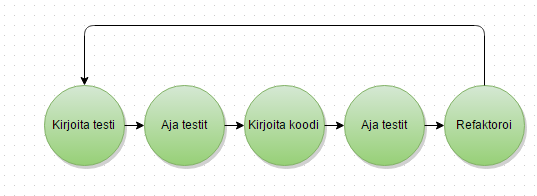
\includegraphics[width=\textwidth]{tdd}
\caption{TDD:n toiminta yksinkertaistettuna.}
\end{figure}

\begin{enumerate}

  \item Kehittäjä tutkii esimerkiksi vaatimusmäärittelyn käyttötapauksia, ja kirjoittaa niiden perusteella testin.

  \item Kehittäjä ajaa testit ja varmistaakseen antaako ohjelma testin vaatiman lopputulokset ilman muutoksia. Testi saattaa myös mennä läpi vaikkei kehittäjä ole mielestään kirjoittanut koodia kyseiselle tapaukselle, tällöin laadittu testi saattaa olla virheellinen antaen aina hyväksytyn tuloksen.

  \item Jos testejä ei läpäisty, siirrytään kirjoittamaan koodia. Kehittäjä täydentää ohjelmaa antamaan hyväksyttävän tuloksen hylättyyn testiin. Lisätyn koodin pitäisi keskittyä ainoastaan testin määrittelemiin toimintoihin, tarkoitus ei ole kirjoittaa muuta toiminnallisuutta.

 \item Testit ajetaan uudestaan. Jos testi yhä epäonnistuu, palataan kohtaan kolme ja koodi parannellaan. Jos testi läpäistään, siirrytään seuraavaan kohtaan.

 \item Kirjoitettu koodi refaktoroidaan. Koodista esimerkiksi poistetaan turha toisto ja mahdollisesti ylipitkiksi kasvaneet metodit pilkotaan. Tämän jälkeen palataan ensimmäiseen kohtaan ja prosessi aloitetaan alusta uudella testillä.

\end{enumerate}

Testivetoisen kehityksen testit kirjoitetaan tutkimaan ohjelman pienimpiä mahdollisia yksikköjä, eli ohjelman osia joita voidaan testata \cite{Crispin06}. Crispinin mukaan pienimmän mahdollisen yksikön määritelmä on kiistanalainen, mutta olio-ohjelmoinnissa sitä on yleisesti pidetty metodina. Testien kirjoittaminen vasta varsinaisen koodin jälkeen voi kestää minuuteista kuukausiin, kun taas test driven developmentia käyttäessä testit ovat käytettävissä välittömästi. \cite{Janzen05}. 

Testivetoisen kehitys siis perustuu testaukseen, mutta se viekkaasti myös vaikuttaa suunnitteluun. Koska testit kirjoitetaan ensin, ohjelmoija joutuu miettimään miten toteuttaa koodi siten, että se on myös testattava. Menetelmä myös  kehottaa refaktoroimaan koodia säännöllisesti jokaisen kierroksen lopussa.

TDD:llä on myös muutamia samankaltaisia sukulaisia, esimerkiksi 
Acceptance Test Driven Development, Behavior-Driven Development ja Story-Test-Driven Development \cite{Turhan10}, mutta niitä ei käsitellä tässä tutkimuksessa tarkemmin.


\section{TDD:n vaikutus laatuun}

Test Driven Development-menetelmästä on tehty useita tutkimuksia. Esimerkiksi Rafique ja kumppanit ovat tutkineet 27 empiiristä ennen helmikuuta 2011 julkaistua tutkimusta aiheesta \cite{Rafique13}. Turhan ja kumppanit löysivät peräti 325 artikkelia, joista he siivilöivät 22 tarkoituksenmukaista tutkimusta \cite{Turhan10}.

Tässä tutkielmassa käsitellään 11 empiiristä tutkimusta TDD:n vaikutuksesta testiryhmän tekemän ohjelman laatuun ja taloudellisuuteen, ja niiden tuloksia arvioidaan seuraavissa kappaleissa. Tutkimuksia ei ole valikoitu esimerkiksi testiryhmän taustan tai kirjoitetun ohjelman ominaisuuksien perusteella, vaan tarkoituksena on ollut valita mahdollisimman yleinen otos. TDD:stä kirjoitettujen artikkelien tuloksia luokitellaan ISO 9126:n määrittelemien sisäisen ja ulkoisen laadun kategorioita soveltamalla, vaikka erilaisia tuloksia onkin vaikea lokeroida luokkien sisälle: onko esimerkiksi virheiden määrä ohjelmassa luotettavuuteen vai toimivuuteen littyvä termi? 


%Tähän erilaisia tutkimuksia, mitä mittareita niissä on käytetty, millaiset tutkimusryhmät, mitä tuloksia


%Toimiiko vai ei?

\subsection{Toimivuus}

Yksikään yhdestätoista tutkimuksesta ei arvioinut tuotetun ohjelman toimivuutta. Yksi ongelma on englanninkielinen termi functionality, jolla usein TDD:tä käsittelevissä artikkeleissa viitataan ohjelman osien, kuten metodien, toimintaan. ISO:n laatustandardi kuitenkin määrittelee toimivuuden ohjelman toimivuudeksi, joten tutkimusten tapa käyttää termiä ei sovellu selkeästi tähän luokkaan. TDD:n väitetyt parannukset ohjelman rakenteen laatuun saattavat vaikuttaa toimivuuteen, mutta mielestäni tutkimukset aiheesta asettuvat loogisemmin muihin laatukategorioihin.

\subsection{Luotettavuus}

Luotettavuus vaikuttaa olevan suosituin laadun osa testivetoista kehitystä käsittelevissä artikkeleissa, ja sitä on tutkittu kymmenessä yhdestätoista tutkielmassa käsitellystä tutkimuksesta. Useat tutkimukset ovat mitanneet TDD:llä tuotetun ohjelmiston laatua testien läpäisyn perusteella, jota voidaan pitää luotettavuuteen liittyvänä tekijänä. Toisaalta ISO:n laatuluokitusten mukaan luotettavuus voidaan ymmärtää myös tarkoittavan virheistä palautumista, eikä niinkään virheiden vähyyttä. ISO 9126-3 kuitenkin esittää koodikattavuuden ja katselmoidusta koodista havaittujen virheiden määrän luotettavuuden mittareina, joten virheiden havaitsemiseen perustuvat tutkimukset ovat tässä osiossa perusteltuja.

Georgen ja Williamsin \cite{George04} tutkimuksessa havaittiin TDD:tä käyttäneiden parien tuottamien ohjelmien läpäisevän 18 prosenttia enemmän tutkijoiden rakentamia testitapauksia kuin kontrolliryhmien. Tutkimuksessa oli kuitenkin ongelmia joiden takia tulosta voidaan pitää kyseenalaisena: Georgen ja Williamsin tutkimuksessa ohjelmat olivat erittäin lyhyitä, pituudeltaan n. 200 riviä, ja suurin osa kontrolliryhmistä ei ollut tehnyt minkäänlaisia testejä ennen ohjelman palautusta tutkijoille.

Wilkersonin ja kumppanit \cite{Wilkerson12} vertailevat TDD:tä koodikatselmointi-menetelmään, jossa erillinen ryhmä arvioi koodia. Tutkijoiden mukaan menetelmillä on selvä ero, katselmointi poistaa ohjelmasta löytyviä virheitä, mutta TDD käsittelee ne jo kehitysvaiheessa. Tutkimuksen tulosten mukaan katselmointia ja TDD:tä yhdistävän ryhmän ohjelmassa oli vähiten virheitä kun taas pelkkää TDD:tä käyttäneellä ryhmällä tulos ei ollut perinteisiä menetelmiä parempi. Wilkersonin ja kumppanien mukaan tutkimuksen neutraali tulos saattaa selittyä TDD-menetelmän liian epämääräisellä määrittelyllä.

Erdogmus, Morisio ja Torchiano \cite{Erdogmus05} tutkivat testivetoista kehitystä verrattuna testien kirjoittamiseen jälkeenpäin (test-last). Tutkimuksen osaanottaneista opiskelijoista TDD:tä käyttäneet olivat kirjoittaneet keskimäärin 28 prosenttia enemmän testejä. Ohjelman laadussa testivetoinen kehitys olikin yllättäen jälkeenpäin testausta huonompi: test-last ryhmän mediaani virheiden määrässä käytettäessä tutkijoiden laatimaa testipakettia oli kymmenen prosenttia pienempi. Tutkijoiden ehdottama selitys TDD:n hieman heikomman laadun johtumisesta ohjelman pienuudesta ja koehenkilöiden erilaisista taitotasoista on perusteltu. Testihenkilöiden tuottama ohjelma oli keilauksen pistelaskujärjestelmä, joka on sen verran yksinkertainen tehtävä, että virheet pystyy helposti löytämään myös ilman yhtäkään automaattista testiä. Causevicin ja kumppanien \cite{Causevic12} tutkimus oli menetelmiltään hyvin samankaltainen kuin Erdogmusin ja kumppanien. Tässäkin tutkimuksessa vertailtiin keilailun pistelaskua suorittavan ohjelman testauksen laatua Test-First ja Test-Last menetelmillä käyttäen testiryhmänä yliopisto-opiskelijoita. Causevicin ja kumppanien tutkimuksessa molempien ryhmien testien laatu oli hyvin samankaltainen, eikä merkittäviä eroja havaittu. Itse ohjelman koodin laadussa oli kuitenkin ero TDD:n hyväksi. Vaikka tutkimukset olivat lähes identtiset,  oli tuloksissa pieni ero. Todennäköisesti ohjelman ja koeryhmien pienuus vaikuttaa Causevicin ja Erdogmusin tutkimuksissa tulokseen enemmän kuin ohjelmointimenetelmä.

 Canfora ja kumppanit \cite{Canfora06} ovat testanneet menetelmää Espanjalaisen IT-yrityksen ammattilaisilla. Tutkijoiden mukaan TDD:n testit eivät ole tilastollisesti merkittävästi tarkempia vesiputousmallilla tuotettuihin verrattuna. Canfora ja kumppanit kuitenkin toteavat olevansa "vakuuttuneita" TDD:n positiivisesta vaikutuksesta laatuun, ja uskovat tulokset olevan merkittävä pidemmässä tutkimuksessa.

Pancur ja Ciglaric \cite{Pancur11} havaitsivat TDD:n tuottavan paremman päätöskattavuuden kuin iteratiivinen Test-Last menetelmä. Mutaatiotestauksessa ja hyväksyttyjen testien määrässä ei havaittu eroa. Myös Munirin ja kumppanien \cite{Munir14} tutkimuksessa päätöskattavuus oli parantanut, mutta tulos ei ollut tilastollisesti merkittävä johtuen liian pienestä koeryhmästä.

Nagappan ja kumppanit \cite{Nagappan08} tutkivat TDD:n vaikutusta laatuun ja tehokkuuteen IBM:n ja Microsoftin ohjelmistotuotannossa. Tutkijat määrittelivät laadun koodin virhetiheydeksi, ja virheiden määrä verrattuna samankaltaisiin projekteihin joissa TDD:tä ei oltu käytetty oli selvästi matalampi. IBM:n projekteissa vähennys oli 40\% ja Microsoftin projekteissa 60-90\%. Tulos on erittäin positiivinen, ja vaikutus selvästi suurempi kuin muissa tässä artikkelissa käsitellyissä tutkimuksissa. Tutkijoiden mukaan tulos saattaa selittyä esimerkiksi projektien vaikeustasossa: TDD ryhmille on saattanut osua helpompia projekteja.

\subsection{Käytettävyys}

Testivetoinen kehitys tuskin vaikuttaa loppukäyttäjän kokemukseen ohjelman laadusta, koska TDD:n prosessi ei varsinaisesti ota kantaa käytettävyyteen. Hellman ja kumppanit \cite{Hellman10} pitävät graafisen käyttöliittymän kehitystä TDD:llä niin vaikeana, että ovat artikkelissaan pyrkineet kehittämään TDD:stä paremmin tehtävään sopivaa muunnosta.

Yksikään tutkielmaan valituista artikkeleista ei ottanut kantaa käytettävyyteen, joten vertailenkin tässä osiossa itse menetelmän käytettävyyttä. TDD:n prosessi on yksinkertainen, joten todennäköisesti aloittelevakin ohjelmoija ymmärtää sen toimintatavat nopeasti. Useissa tutkimuksissa käyttäjien omia näkemyksiä menetelmästä on selvitetty, mutta tähän osioon on valikoitu vain tutkimuksia joissa TDD:n käytön oikeellisuutta on mitattu muutenkin kuin käyttäjien mielipiteiden perusteella.

Latorren \cite{Latorre14} tutkimuksessa mittauksien mukaan menetelmä oli helppo oppia, varsinkin kehittyneet ja keskitason ohjelmoijat oppivat sen nopeasti.

Oulun yliopiston Fucci, Turhan ja Oivo \cite{Fucci14} tutkivat TDD:n prosessin noudattamisen tarkkuuden vaikutusta laatuun. Fuccin ja kumppaneiden mukaan TDD:tä koskevissa tutkimuksissa menetelmän seuraamisen arviointi ei ole tehty tarpeeksi, vaikka se saattaa oleellisesti vaikuttaa tuloksiin. Tutkimuksen TDD:tä käyttäneiden opiskelijoiden tuottama laatu ei ollut ollut sidoksissa siihen, kuinka hyvin he noudattivat menetelmää. Tutkijat havaitsivat opiskelijoiden usein keskittyvän vain testien kirjoittamiseen ja jättävän refaktorointivaiheen kokonaan pois. Fucci ja kumppanit kyseenalaistavat TDD:n opettelun ja noudattamisen hyödyn, mutta pitävät mahdollisena hyötyjen tulevan esiin pidemmissä tutkimuksissa.

\subsection{Tehokkuus}

ISO 9126 mittaa tehokkuutta mittareilla kuten vasteaika ja muistinkäyttö. Tutkimus testivetoisen kehityksen vaikutuksesta ohjelmistojen tehokkuuten ei selvästi ole ollut kovin suosittu tutkimuskohde, koska yksikään yhdestätoista tutkimuksesta ei sitä noteerannut. Tutkimusta itse menetelmän tehokkuudesta löytyy runsaasti, mutta se asettuu paremmin omaan osioonsa TDD:n taloudellisuudesta. TDD:n toimintavat eivät suoranaisesti vaikuta ohjelman sellaiseen suunnitteluun, joka parantaisi ohjelman resurssienkäyttöä, vaan siihen tarvittaisiin tarkempia rakenteen suunnittelun ohjeita. TDD:n etuna esitetty selkeämpi ja modulaarinen rakenne tuskin suoraan vaikuta ISO-standardissa esiteltyjen tehokkuuden mittareiden tuloksiin.

\subsection{Ylläpidettävyys}

Testivetoisen kehityksen vaikutus ohjelman rakenteeseen vaikuttanee myös sen ylläpidettävyyteen, koska modulaarinen ja selkeä ohjelmakoodi on helpommin laajennettavaa ja korjattavaa. Ohjelman rakenteen mittaaminen tehokkaasti vaikuttaa tutkimusten perusteella vaikeammalta kuin esimerkiksi luotettavuuden mittaaminen; virheitä on helpompi laskea kuin arvioida rakenteeseen liittyviä ominaisuuksia. Koska mahdolliset uudet virheet löydetään helpommini kattavan testipaketin avulla kuin ilman, testien laatu ja luotettavuus ovat myös selkeästi ylläpidettävyyteen ja laajennettavuuteen liittyviä tekijöitä, joten näitä laadun osa-alueita koskevilla tutkimuksilla on yhteys.

Siniaalto ja Abrahamsson \cite{Siniaalto07} tutkivat TDD:n vaikutusta ohjelmiston laatuun. Tutkijat käyttivät mittareina tässäkin tutkielmassa esiteltyjä Chidamberin ja Kemenerin laadun mittareita, poislukien rivien määrä. Siniaalto ja Abrahamsson vertasi TDD:llä tehtyä ohjelmaa kahteen ohjelmaan, joissa testaus oli tehty vasta koodin jälkeen. Ohjelmien tulokset olivat samankaltaisia, mutta TDD:n oli luokkien metodien välisen koheesion metriikassa selvästi muita huonompi. 

Pancurin ja Ciglaricin tutkimuksessa \cite{Pancur11} TDD tuotti paremman syklomaattisen kompleksisuuden verrattuna testaamiseen jälkeenpäin, mutta vaikutus oli liian pieni ollakseen tilastollisesti merkittävä. Syklomaattinen kompleksisuus on Thomas J. McCaben kehittämä mittari \cite{McCabe76}, joka arvioi ohjelman lähdekoodissa olevien erillisten polkun määrää. Korkea määrä polkuja on merkki rakenteesta, jota on McCaben mukaan vaikea testata ja ylläpitää. Munirin ja kumppanit \cite{Munir14} tarkastelivat myös McCaben mittaria, eikä ero verrattuna Test-Lastiin ollut tilastollisesti merkittävä.

\subsection{Siirrettävyys}

Valittuihin artikkeleihin ei osunut tutkimuksia joissa oltaisiin tutkittu TDD:n vaikutusta ohjelmiston siirrettävyyteen. Testivetoisen kehityksen prosessi ei sivua siirrettävyyteen vaikuttavia tekijöitä, joten tutkimuksen vähäisyys oli odotettavissa.
Samaan tapaan kuin käytettävyyttä tutkiessa, onkin ehkä järkevämpää tutkia miten itse TDD:n tekniikka soveltuu eri alustoilla. Tästäkään aiheesta en ole löytänyt tutkimuksia, mutta luultavasti TDD toimii kaikilla alustoilla ja ohjelmointikielillä joissa voi kirjoittaa testejä. Tämä kriteeri on niin löysä, että TDD:tä voi todennäköisesti käyttää lähes missä tahansa ohjelmointitilanteessa.

%Integraatiotestauksessakin varmaan ongelmia, löytää vain lähteen


\subsection{Vaikutus taloudellisuuteen}

George ja Williams \cite{George04} havaitsivat TDD:tä käyttäneiden pariohjelmoijien käyttäneen 16 prosenttia enemmän aikaa tehtävän suorittamiseen kuin tavanomaista vesiputousmalli noudattanut kontrolliryhmä. Toisaalta suurin osa kontrolliryhmistä oli jättänyt testitapaukset tekemättä, joten tuloksesta ei voi tehdä suuria johtopäätöksiä.

Ohjelman rakenteeseen keskittyneessä tutkimuksessaan Siniaalto ja Abrahamsson \cite{Siniaalto07} toteavat TDD:n tuottavan korkean testikattavuuden ilman tuottavuuden kärsimistä.

Erdogmus ja kumppanit \cite{Erdogmus05} havaitsivat testivetoista kehitystä käyttäneiden oppilaiden olleen tehokkaampia kuin jälkeenpäin testit rakentaneet oppilaat. Tehokkuuden kasvussa oli vaihtelua riippuen ohjelmoijan taidoista: positiivinen vaikutus tehokkuuteen oli suurin taitavilla ohjelmoijilla. Erdogmus ja kumppanit määrittelivät tehokkuuden hyväksyttävästi läpäistyjen käyttötapausten määränä verrattuna aikaan. Tutkimuksessa kuitenkin havaittiin myös pieni negatiivinen vaikutus ohjelman laatuun TDD:tä käyttäessä, joten käytetty laadun määritelmä ei ehkä ollut täysin tutkimukseen sopiva, vaan myös laatu olisi pitänyt laskea mukaan taloudellisuuteen.

Canforan ja kumppanit \cite{Canfora06} tilastollisen analyysin mukaan testivetoinen kehitys vaatii enemmän aikaa kuin jälkeenpäin testaaminen, mutta tutkijat uskovat TDD:n paremman laadun parantavan taloudellisuutta.

Pancur ja Ciglaric \cite{Pancur11} olivat tutkimuksessaan verranneet TDD:tä iteratiiviseen Test-Last menetelmään. Test-Last kontrolliryhmälle määrätty toimintapa muistutti hyvin paljon TDD:tä, ainoastaan testien ja koodin järjestystä prosessilla oli muutettu. Tutkijat päättelivät pieniin iteraatiohin perustuvan suunnittelun vaikuttavan merkittävästi tuloksiin, johon heidän kontrolliryhmälleen laatima prosessi kannustaa. Pancurin ja Ciglaricin tutkimusten mukaan vaikutus tehokkuuteen, eli tässä tapauksessa tuotettuihin testeihin per tunti,  oli positiivinen, mutta liian pieni ollakseen tilastollisesti merkittävä.

Madeyski ja Szala \cite{Madeyski07} havaitsivat TTD:tä käyttävän ohjelmoijan olevan tehokkaampi kuin käyttäessä Test-Last menetelmää. Kiinnostavaa tässä tutkimuksessa on se, että koehenkilönä oli vain yksi kokenut ohjelmoija, joka toteutti ohjelmaa vaihdellen menetelmiä. Tutkimuksessa oli useita mielenkiintoisia piirteitä: yhden ohjelmoijan tehokkuuden mittaus pitkällä aikavälillä, tässä ohjelman toteutus kesti 122 tuntia, on kiinnostava näkökulma. Tutkijat myös mittasivat kuinka pitkän ajan käyttötapauksen kehityksestä ohjelmoija oli passiivinen eikä kirjoittanut koodia, eli kuinka pitkään hän luki koodia tai etsi bugeja. Yhden hengen koeryhmää ei mielestäni voi pitää mitenkään tieteellisesti uskottavana, joten haluaisin nähdä saman tutkimuksen isommalla koeryhmällä.

Nagappan ja kumppanit \cite{Nagappan08} tutkivat TDD:tä yrityskäytössä. TDD:tä käyttäneet ryhmät käyttivät 15 \%-35 \% enemmän aikaa projektin tuottamiseen, mutta laatu oli selkeästi parempaa. Tutkijoiden mukaan suuri parannus laadussa oli merkittävämpi kuin lasku tuotannon nopeudessa, joten menetelmä on taloudellisempi. Myös yrityksen ohjelmointiryhmät olivat samaa mieltä TDD:n paremmasta taloudellisuudesta.

\subsection{Kehittäjien mielipiteitä menetelmästä}

Eräissä artikkeleissa on tehty myös kvalitatiivista tutkimusta, esimerkiksi selvittämällä testihenkilöiden henkilökohtaisia näkemyksiä testivetoisen kehityksen toimivuudesta.

Georgen ja Williamsin \cite{George04} tutkimuksen osaanottajat pitivät menetelmää erityisen hyvänä koodin laadun ja ohjelmoijan tuottavuuden kannalta, mutta oikeaan "mielenlaatuun" pääsemistä oli pidetty vaikeana. Tutkimusryhmänä tutkimuksessa oli 24 ammattilaisohjelmoijaa.

Latorren \cite{Latorre14} tutkimuksessa testivetoisen kehityksen oppimisen vaativuudesta 24 ammattilaista 25:stä piti menetelmää helppona oppia, ja tutkijan mittausten perusteella he myös käyttivät sitä oikein.

Ljubljanan yliopistossa tehdyssä Pancurin ja Ciglaricin\cite{Pancur11} tutkimuksessa menetelmää pidettiin vaikeasti opittavana verrattuna testien kirjoittamiseen jälkeenpäin. Koeryhmänä toimineet neljännen vuoden tietojenkäsittelytieteen opiskelijat eivät tutkijoiden mukaan mahdollisesti hallinneet menetelmää tarpeeksi hyvin kymmenen viikon harjoittelun jälkeen.

Munirin ja kumppanien \cite{Munir14} tutkimuksessa ammattilaiset eivät pitäneet TDD:stä. Kyselytutkimuksessa menetelmää pidettiin vaikeana oppia sekä vaativan enemmän aikaa ja itsekuria. Suurin osa 15:sta TDD:tä tutkimuksessa käyttäneestä koehenkilöistä ei ollut ennen käyttänyt menetelmää. Ammattilaiset pitivät testien kirjoittamista ensin ongelmallisena, koska kehittäjän ja asiakkaan näkökulmasta varsinainen ohjelman toiminnallisuus nähdään arvokkaampana kuin testit. Munirin ja kumppanien mukaan TDD:n tehokas käyttö vaatii harjoittelua ja hyvää testienkirjoitustaitoa.


\subsection{Kirjallisuuskatsaukset}

Lyhyessä kandidaatintutkielmassa ei tietenkään voi käsitellä kaikkia maailman tutkimuksia TDD:stä. Onneksi TDD:stä on tehty myös meta-analyysia, jota tutkimalla saamme paremman kuvan menetelmän vaikutuksista.

Rafiquen ja Misic \cite{Rafique13} ovat analysoineet testivetoisen kehityksen vaikutusta laatuun ja tehokkuuteen. Tutkimuksessa laatu on määritelty virheiden määränä verrattuna koodin määrään ja tehokkuus tuotettuna koodina verrattuna aikaan, tutkimukset joissa on tutkittu TDD:tä muilla mittareilla on jätetty pois analyysista. Ohjelman rakenteen laatu on jätetty pois tutkitumuksesta, koska tutkijoiden mukaan suuunnittelun laatua on erittäin vaikea arvioida.  Rafique ja Misic ovat tarkoituksella valikoineet ainoastaan tutkimuksia joissa TDD:tä on verrattu tavanomaisiin kehitysmenetelmiin, kuten vesiputousmalliin ja iteratiiviseen Test-Last menetelmään. Myös tutkimukset joissa TDD:n prosessia ei ole noudatettu tarkasti on jätetty pois analyysista. Tutkimukset oli tehty opiskelija- ja ammattilaisryhmillä.

Rafique ja Misic toteavat analyysin tuloksien osoittavan TDD:n tuottavan pienen parannuksen laatuun, mutta tehokkuudessa tulos ei ole ratkaiseva. Teollisessa kontekstissa positiivinen vaikutus laatuun oli selvästi suurempi kuin akatemisessa, mutta toisaalta ammattilaisilla myös tehokkuus oli matalampi.





\subsection{Johtopäätökset}



Tutkimuksia-osiossa käsitellyt tutkimukset eivät anna testivetoisesta kehityksen hyödyistä selkeää kuvaa. Tulokset ovat useimmiten neutraaleja tai lievästi positiivisia.
  Taulukkoon 1 on koottu tässä tutkielmassa käsiteltyjä tutkimuksia. Positiiviset tulokset on merkitty plussalla, negatiiviset miinuksella, neutraalit yhtäsuuruusmerkillä ja tyhjällä ne tutkimukset joissa aiheeseen ei otettu kantaa. Luokittelut perustuvat tutkimusten tekijöiden näkemykseen, ja niissä on hieman tulkinnan varaa. Taulukkoon on valikoitu ne laadun osa-alueet joihin tutkimukset ottivat kantaa, tälläisiksi luokitteltiin luotettavuus, ylläpidettävyys ja taloudellisuus. Lisäksi käyttäjien mielipide menetelmästä on kiinnostava "laatunäkökulma".

\begin{table}
\begin{tabular}{ l  c  c  c  c}
\toprule
  Tutkimus & Luotettavuus & Ylläpidettävyys & Taloudellisuus & Mielipide \\
\midrule
\cite{George04} 	& + &  & = & + \\ 
\cite{Wilkerson12} 	& = &  &   &   \\ 
\cite{Erdogmus05} 	& - &  	& + &   \\ 
\cite{Causevic12} 	& = & + &   &   \\
\cite{Canfora06} 	& = &  & = &   \\ 
\cite{Pancur11} 	& + & = & = & - \\
\cite{Munir14} 	& = & = &   & - \\ 
\cite{Nagappan08} 	& + &  & + &   \\ 
\cite{Siniaalto07} 	& = & - & + &   \\ 
\cite{Madeyski07} 	&   &   & + &   \\ 
\cite{Latorre14}	&   &   & + & + \\ 
\bottomrule
\end{tabular}
\caption{Tulosten yhteenveto. Mielipide-sarakkeella tarkoitetaan kehittäjien näkemystä TDD:stä}
\end{table}


Parempi luotettavuus on esiintynyt TDD:tä käsittelevissä artikkeleissa sen tärkeimpänä ehdotettuna hyötynä. Luotettavuus ei kuitenkaan ole erityisen voimakkaasti tullut esille näissä tutkimuksissa, vaan neutraaleja tuloksia on enemmän kuin positiivisia. Käsittellyt tutkimukset olivat  kestoltaan ja laajuudeltaan melko lyhyitä, joten menetelmä ei ehkä ollut niissä vahvimmillaan. Useissa tutkimuksissa onkin mainittu syynä heikoille tuloksille tutkimusten pieni koko. 

Ylläpidettävyydessä useat tutkimukset kärsivät liian pienestä tutkimuksen koosta, molemmissa neutraaliksi merkityssä tutkimuksessa paremmasta laadusta oli merkkejä, mutta tulos ei tutkijoiden mukaan ollut tilastollisesti merkittävä johtuen pienestä otoksesta. Siniahon ja Abrahamssonin tutkimuksessa ohjelman rakenteessa oli havaittu negatiivinen vaikutus.

Taloudellisuudessa tulokset ovat yllättävän positiivisia. On perusteltua päätellä paremman laadun ja pidemmän prosessin johtavan neutraaliin vaikutukseen, mutta käsitellyissä tutkimuksissa vaikutus onkin selkeästi positiivinen. Osassa tutkimuksista kirjoittajat havaitsivat ohjelman valmistuvan hitaammin, mutta arvioivat laatuvaikutuksen olevan suurempi. Rafiquen ja Misicin meta-analyysissä vaikutuksen taloudellisuuteen on kuitenkin havaittu olevan neutraali ja ammattilaisilla jopa negatiivinen. Tutkielmaan valitut tutkimukset olivat kuitenkin melko lyhyitä, joten ehkä TDD tuottaa paremman taloudellisuuden varsinkin pienissä ohjelmissa.

Mielipide-sarake on lisätty taulukkoon, koska kehittäjien näkemys menetelmästä saattaa vaikuttaa tuloksiin ja ohjelman laatuun. Vanhat toimintatavat saattavat tuntua paremmilta, koska ohjelmointi "takaperin" pakottaa ohjelmoijan toimimaan uudella tavalla. Jos menetelmä vaikuttaa vastenmieliseltä, vaikuttanee se myös vaikuttaa työnjälkeen negatiivisesti. Otos on kuitenkin sen verran pieni, ettei näistä tuloksista voi vetää johtopäätöksiä. 

\section{Yhteenveto}

Artikkelissa tutkittiin TDD:n vaikutusta laatuun ja tehokkuuteen. Laatu määriteltiin käyttämällä apuna ISO 9126 standardin laadun osa-alueita. Tehokkuuden arviointiin käytettiin tarkasteltujen tutkimusten käsitystä tehokkuudesta, eli useimmiten tuotetun koodin määrää verrattuna aikaan. Tutkimusten tulokset aseteltiin parhaiten soveltuviin kategorioihin ja niitä verrattiin meta-analyysien tuloksiin. Useimmin käsitellyiksi ISO-standardin kategorioiksi nousivat luotettavuus ja ylläpidettävyys.

Luotettavuuden havaittiin paranevan hieman TDD:tä käytettäessä. Tehokkuudessa käsitellyt tutkimukset osoittivat parannusta, mutta tulos eroaa meta-analyyseistä. Ylläpidettävyydessä tulos oli neutraali.



% --- References ---
%
% bibtex is used to generate the bibliography. The babplain style
% will generate numeric references (e.g. [1]) appropriate for theoretical
% computer science. If you need alphanumeric references (e.g [Tur90]), use
%
% \bibliographystyle{babalpha-lf}
%
% instead.

\bibliographystyle{babalpha-lf}
\bibliography{../ref}


% --- Appendices ---

% uncomment the following

% \newpage
% \appendix
% 
% \section{Esimerkkiliite}

\end{document}